\documentclass[twoside]{book}

% Packages required by doxygen
\usepackage{fixltx2e}
\usepackage{calc}
\usepackage{doxygen}
\usepackage[export]{adjustbox} % also loads graphicx
\usepackage{graphicx}
\usepackage[utf8]{inputenc}
\usepackage{makeidx}
\usepackage{multicol}
\usepackage{multirow}
\PassOptionsToPackage{warn}{textcomp}
\usepackage{textcomp}
\usepackage[nointegrals]{wasysym}
\usepackage[table]{xcolor}

% Font selection
\usepackage[T1]{fontenc}
\usepackage[scaled=.90]{helvet}
\usepackage{courier}
\usepackage{amssymb}
\usepackage{sectsty}
\renewcommand{\familydefault}{\sfdefault}
\allsectionsfont{%
  \fontseries{bc}\selectfont%
  \color{darkgray}%
}
\renewcommand{\DoxyLabelFont}{%
  \fontseries{bc}\selectfont%
  \color{darkgray}%
}
\newcommand{\+}{\discretionary{\mbox{\scriptsize$\hookleftarrow$}}{}{}}

% Page & text layout
\usepackage{geometry}
\geometry{%
  a4paper,%
  top=2.5cm,%
  bottom=2.5cm,%
  left=2.5cm,%
  right=2.5cm%
}
\tolerance=750
\hfuzz=15pt
\hbadness=750
\setlength{\emergencystretch}{15pt}
\setlength{\parindent}{0cm}
\setlength{\parskip}{3ex plus 2ex minus 2ex}
\makeatletter
\renewcommand{\paragraph}{%
  \@startsection{paragraph}{4}{0ex}{-1.0ex}{1.0ex}{%
    \normalfont\normalsize\bfseries\SS@parafont%
  }%
}
\renewcommand{\subparagraph}{%
  \@startsection{subparagraph}{5}{0ex}{-1.0ex}{1.0ex}{%
    \normalfont\normalsize\bfseries\SS@subparafont%
  }%
}
\makeatother

% Headers & footers
\usepackage{fancyhdr}
\pagestyle{fancyplain}
\fancyhead[LE]{\fancyplain{}{\bfseries\thepage}}
\fancyhead[CE]{\fancyplain{}{}}
\fancyhead[RE]{\fancyplain{}{\bfseries\leftmark}}
\fancyhead[LO]{\fancyplain{}{\bfseries\rightmark}}
\fancyhead[CO]{\fancyplain{}{}}
\fancyhead[RO]{\fancyplain{}{\bfseries\thepage}}
\fancyfoot[LE]{\fancyplain{}{}}
\fancyfoot[CE]{\fancyplain{}{}}
\fancyfoot[RE]{\fancyplain{}{\bfseries\scriptsize Generated by Doxygen }}
\fancyfoot[LO]{\fancyplain{}{\bfseries\scriptsize Generated by Doxygen }}
\fancyfoot[CO]{\fancyplain{}{}}
\fancyfoot[RO]{\fancyplain{}{}}
\renewcommand{\footrulewidth}{0.4pt}
\renewcommand{\chaptermark}[1]{%
  \markboth{#1}{}%
}
\renewcommand{\sectionmark}[1]{%
  \markright{\thesection\ #1}%
}

% Indices & bibliography
\usepackage{natbib}
\usepackage[titles]{tocloft}
\setcounter{tocdepth}{3}
\setcounter{secnumdepth}{5}
\makeindex

% Hyperlinks (required, but should be loaded last)
\usepackage{ifpdf}
\ifpdf
  \usepackage[pdftex,pagebackref=true]{hyperref}
\else
  \usepackage[ps2pdf,pagebackref=true]{hyperref}
\fi
\hypersetup{%
  colorlinks=true,%
  linkcolor=blue,%
  citecolor=blue,%
  unicode%
}

% Custom commands
\newcommand{\clearemptydoublepage}{%
  \newpage{\pagestyle{empty}\cleardoublepage}%
}

\usepackage{caption}
\captionsetup{labelsep=space,justification=centering,font={bf},singlelinecheck=off,skip=4pt,position=top}

%===== C O N T E N T S =====

\begin{document}

% Titlepage & ToC
\hypersetup{pageanchor=false,
             bookmarksnumbered=true,
             pdfencoding=unicode
            }
\pagenumbering{roman}
\begin{titlepage}
\vspace*{7cm}
\begin{center}%
{\Large My Project }\\
\vspace*{1cm}
{\large Generated by Doxygen 1.8.11}\\
\end{center}
\end{titlepage}
\clearemptydoublepage
\tableofcontents
\clearemptydoublepage
\pagenumbering{arabic}
\hypersetup{pageanchor=true}

%--- Begin generated contents ---
\chapter{File Index}
\section{File List}
Here is a list of all files with brief descriptions\+:\begin{DoxyCompactList}
\item\contentsline{section}{\hyperlink{Lab1_8c}{Lab1.\+c} }{\pageref{Lab1_8c}}{}
\end{DoxyCompactList}

\chapter{File Documentation}
\hypertarget{Recurrsion_8cpp}{}\section{Recurrsion.\+cpp File Reference}
\label{Recurrsion_8cpp}\index{Recurrsion.\+cpp@{Recurrsion.\+cpp}}
{\ttfamily \#include $<$iostream$>$}\\*
Include dependency graph for Recurrsion.\+cpp\+:
\nopagebreak
\begin{figure}[H]
\begin{center}
\leavevmode
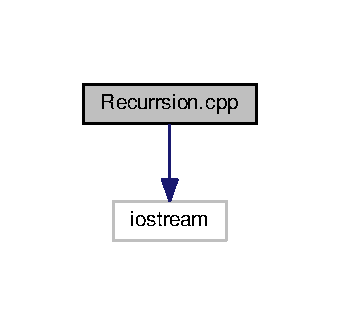
\includegraphics[width=163pt]{Recurrsion_8cpp__incl}
\end{center}
\end{figure}
\subsection*{Functions}
\begin{DoxyCompactItemize}
\item 
void \hyperlink{Recurrsion_8cpp_af5d44dbdfddbc984d7a65c6fccefe7ac}{write\+Line} (char c, int n)
\item 
void \hyperlink{Recurrsion_8cpp_a7cd55c1bc6e4c5fba33168b19f285a7a}{write\+Block} (char c, int m, int n)
\item 
int \hyperlink{Recurrsion_8cpp_afdfc604aec5ef288aceb05f598f8dd9c}{factorial\+\_\+01} (int n)
\item 
void \hyperlink{Recurrsion_8cpp_a5a81ff59cd01a2d0b76e26f835130f0e}{factorial\+\_\+02} (int n, int \&f)
\item 
int \hyperlink{Recurrsion_8cpp_ae66f6b31b5ad750f1fe042a706a4e3d4}{main} ()
\end{DoxyCompactItemize}


\subsection{Function Documentation}
\index{Recurrsion.\+cpp@{Recurrsion.\+cpp}!factorial\+\_\+01@{factorial\+\_\+01}}
\index{factorial\+\_\+01@{factorial\+\_\+01}!Recurrsion.\+cpp@{Recurrsion.\+cpp}}
\subsubsection[{\texorpdfstring{factorial\+\_\+01(int n)}{factorial_01(int n)}}]{\setlength{\rightskip}{0pt plus 5cm}int factorial\+\_\+01 (
\begin{DoxyParamCaption}
\item[{int}]{n}
\end{DoxyParamCaption}
)}\hypertarget{Recurrsion_8cpp_afdfc604aec5ef288aceb05f598f8dd9c}{}\label{Recurrsion_8cpp_afdfc604aec5ef288aceb05f598f8dd9c}

\begin{DoxyCode}
57 \{
58    \textcolor{keywordtype}{int} fact = 1; \textcolor{comment}{//fact must start at 1 for when n=1                                                       
                                                                                                       }
59    \textcolor{keywordflow}{if}(n>1) \textcolor{comment}{//stopping case}
60       fact = (n*\hyperlink{Recurrsion_8cpp_afdfc604aec5ef288aceb05f598f8dd9c}{factorial\_01}(n-1));
61    \textcolor{keywordflow}{return} fact;
62 \}
\end{DoxyCode}
\index{Recurrsion.\+cpp@{Recurrsion.\+cpp}!factorial\+\_\+02@{factorial\+\_\+02}}
\index{factorial\+\_\+02@{factorial\+\_\+02}!Recurrsion.\+cpp@{Recurrsion.\+cpp}}
\subsubsection[{\texorpdfstring{factorial\+\_\+02(int n, int \&f)}{factorial_02(int n, int &f)}}]{\setlength{\rightskip}{0pt plus 5cm}void factorial\+\_\+02 (
\begin{DoxyParamCaption}
\item[{int}]{n, }
\item[{int \&}]{f}
\end{DoxyParamCaption}
)}\hypertarget{Recurrsion_8cpp_a5a81ff59cd01a2d0b76e26f835130f0e}{}\label{Recurrsion_8cpp_a5a81ff59cd01a2d0b76e26f835130f0e}

\begin{DoxyCode}
68 \{
69    f=1; \textcolor{comment}{//f must start at 1 for when n=1                                                                   
                                                                                                       }
70    \textcolor{keywordflow}{if}(n>1) \textcolor{comment}{//stopping case                                                                                 
                                                                                                       }
71       \hyperlink{Recurrsion_8cpp_a5a81ff59cd01a2d0b76e26f835130f0e}{factorial\_02}(n-1, f); \textcolor{comment}{//f is called my reference so that its value is changed for each
       function call                                                                                                 
       }
72    f*=n;
73 \}
\end{DoxyCode}
\index{Recurrsion.\+cpp@{Recurrsion.\+cpp}!main@{main}}
\index{main@{main}!Recurrsion.\+cpp@{Recurrsion.\+cpp}}
\subsubsection[{\texorpdfstring{main()}{main()}}]{\setlength{\rightskip}{0pt plus 5cm}int main (
\begin{DoxyParamCaption}
{}
\end{DoxyParamCaption}
)}\hypertarget{Recurrsion_8cpp_ae66f6b31b5ad750f1fe042a706a4e3d4}{}\label{Recurrsion_8cpp_ae66f6b31b5ad750f1fe042a706a4e3d4}

\begin{DoxyCode}
17 \{
18    \textcolor{keywordtype}{int} f;
19    \hyperlink{Recurrsion_8cpp_af5d44dbdfddbc984d7a65c6fccefe7ac}{writeLine}(\textcolor{charliteral}{'*'}, 5);
20    cout << endl << endl;
21 
22    \hyperlink{Recurrsion_8cpp_a7cd55c1bc6e4c5fba33168b19f285a7a}{writeBlock}(\textcolor{charliteral}{'$'}, 3, 5);
23 
24    cout << \textcolor{stringliteral}{"8! = "} << \hyperlink{Recurrsion_8cpp_afdfc604aec5ef288aceb05f598f8dd9c}{factorial\_01}(8) << endl << endl;
25    cout << \textcolor{stringliteral}{"5! = "} << \hyperlink{Recurrsion_8cpp_afdfc604aec5ef288aceb05f598f8dd9c}{factorial\_01}(5) << endl << endl;
26    cout << \textcolor{stringliteral}{"12! = "} << \hyperlink{Recurrsion_8cpp_afdfc604aec5ef288aceb05f598f8dd9c}{factorial\_01}(12) << endl << endl;
27 
28    \hyperlink{Recurrsion_8cpp_a5a81ff59cd01a2d0b76e26f835130f0e}{factorial\_02}(8, f);
29    cout << \textcolor{stringliteral}{"8! = "} << f << endl << endl;
30    \hyperlink{Recurrsion_8cpp_a5a81ff59cd01a2d0b76e26f835130f0e}{factorial\_02}(5, f);
31    cout << \textcolor{stringliteral}{"5! = "} << f << endl << endl;
32    \hyperlink{Recurrsion_8cpp_a5a81ff59cd01a2d0b76e26f835130f0e}{factorial\_02}(12, f);
33    cout << \textcolor{stringliteral}{"12! = "} << f << endl << endl;
34 
35    \textcolor{keywordflow}{return} 0;
36 \}
\end{DoxyCode}


Here is the call graph for this function\+:
\nopagebreak
\begin{figure}[H]
\begin{center}
\leavevmode
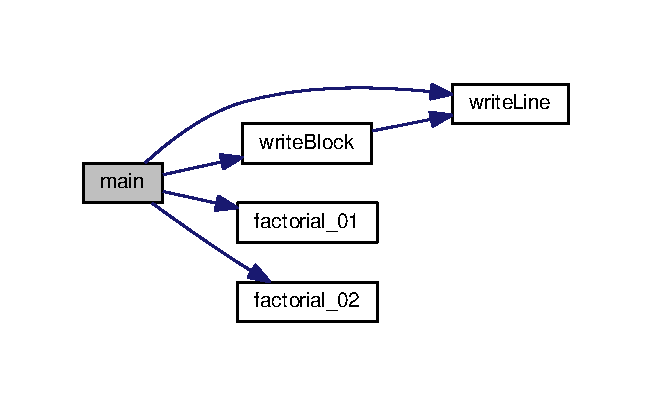
\includegraphics[width=313pt]{Recurrsion_8cpp_ae66f6b31b5ad750f1fe042a706a4e3d4_cgraph}
\end{center}
\end{figure}


\index{Recurrsion.\+cpp@{Recurrsion.\+cpp}!write\+Block@{write\+Block}}
\index{write\+Block@{write\+Block}!Recurrsion.\+cpp@{Recurrsion.\+cpp}}
\subsubsection[{\texorpdfstring{write\+Block(char c, int m, int n)}{writeBlock(char c, int m, int n)}}]{\setlength{\rightskip}{0pt plus 5cm}void write\+Block (
\begin{DoxyParamCaption}
\item[{char}]{c, }
\item[{int}]{m, }
\item[{int}]{n}
\end{DoxyParamCaption}
)}\hypertarget{Recurrsion_8cpp_a7cd55c1bc6e4c5fba33168b19f285a7a}{}\label{Recurrsion_8cpp_a7cd55c1bc6e4c5fba33168b19f285a7a}

\begin{DoxyCode}
48 \{
49    \textcolor{keywordflow}{if}(m>1) \textcolor{comment}{//stopping case                                                                                 
                                                                                                       }
50       \hyperlink{Recurrsion_8cpp_a7cd55c1bc6e4c5fba33168b19f285a7a}{writeBlock}(c, m-1, n);
51    \hyperlink{Recurrsion_8cpp_af5d44dbdfddbc984d7a65c6fccefe7ac}{writeLine}(c, n);
52    cout << endl << endl;
53 \}
\end{DoxyCode}


Here is the call graph for this function\+:
\nopagebreak
\begin{figure}[H]
\begin{center}
\leavevmode
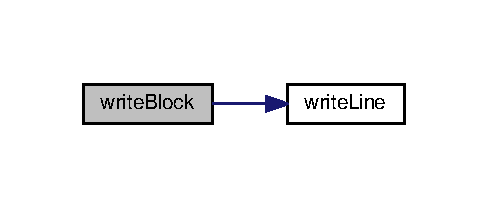
\includegraphics[width=234pt]{Recurrsion_8cpp_a7cd55c1bc6e4c5fba33168b19f285a7a_cgraph}
\end{center}
\end{figure}


\index{Recurrsion.\+cpp@{Recurrsion.\+cpp}!write\+Line@{write\+Line}}
\index{write\+Line@{write\+Line}!Recurrsion.\+cpp@{Recurrsion.\+cpp}}
\subsubsection[{\texorpdfstring{write\+Line(char c, int n)}{writeLine(char c, int n)}}]{\setlength{\rightskip}{0pt plus 5cm}void write\+Line (
\begin{DoxyParamCaption}
\item[{char}]{c, }
\item[{int}]{n}
\end{DoxyParamCaption}
)}\hypertarget{Recurrsion_8cpp_af5d44dbdfddbc984d7a65c6fccefe7ac}{}\label{Recurrsion_8cpp_af5d44dbdfddbc984d7a65c6fccefe7ac}

\begin{DoxyCode}
40 \{
41    \textcolor{keywordflow}{if}(n>1) \textcolor{comment}{//stopping case                                                                                 
                                                                                                       }
42       \hyperlink{Recurrsion_8cpp_af5d44dbdfddbc984d7a65c6fccefe7ac}{writeLine}(c, n-1);
43    cout << c;
44 \}
\end{DoxyCode}

%--- End generated contents ---

% Index
\backmatter
\newpage
\phantomsection
\clearemptydoublepage
\addcontentsline{toc}{chapter}{Index}
\printindex

\end{document}
